%----------------------------------------------------------------------------------------
%	PACKAGES AND OTHER DOCUMENT CONFIGURATIONS
%----------------------------------------------------------------------------------------

\documentclass{article}
\usepackage{amsmath,amsthm}
\usepackage{amsfonts}
\usepackage{fancyhdr} % Required for custom headers
\usepackage{extramarks} % Required for headers and footers
\usepackage{graphicx} % Required to insert images
\usepackage[outdir=./figures/]{epstopdf} 
\epstopdfDeclareGraphicsRule{.pdf}{png}{.png}{convert -density 300 #1 \OutputFile}
\usepackage{pdfpages}
\usepackage{booktabs}
\usepackage{caption}
\usepackage{float}
\usepackage{hyperref}
% Margins
\topmargin=-0.45in
\evensidemargin=0in
\oddsidemargin=0in
\textwidth=6.5in
\textheight=9.0in
\headsep=0.25in 

\linespread{1.1} % Line spacing

% Set up the header and footer
\pagestyle{fancy}
\lhead{\hmwkAuthorName} % Top left header
\chead{\hmwkClass\ : \hmwkTitle} % Top center header
\rhead{\firstxmark} % Top right header
\renewcommand\headrulewidth{0.4pt} % Size of the header rule

\hypersetup{colorlinks=true,urlcolor=blue}
   
%----------------------------------------------------------------------------------------
%	NAME AND CLASS SECTION
%----------------------------------------------------------------------------------------

\newcommand{\hmwkTitle}{Homework\ \#5} % Assignment title
\newcommand{\hmwkClass}{19-704} % Course/class
\newcommand{\hmwkClassInstructor}{} % Teacher/lecturer
\newcommand{\hmwkAuthorName}{Patrick Sheehan} % Your name

%----------------------------------------------------------------------------------------
\begin{document}
\hyperref{https://github.com/patricksheehan/19704}{}{}{Git repository for code for this assignment}

\section{Histograms/Tables: ``...Histograms.R"}
\subsection{Students in each school}
To create the histogram for the number of students in each school, I first had to generate the data since it is not directly included. While there are many ways to do this, I settled on an implementation which counted the number of observations which corresponded to each school. This sum is equivalent to the number of students in each school since each observation represents a unique student. To get the histogram, I used R's standard \verb|hist| function with Scott's rule bin breaks. While I would typically use a discrete-oriented histogram function, the number of schools was not large enough to result in a continuous approximation. The result is in Figure \ref{hist1}.

\begin{figure}[H]
\centering
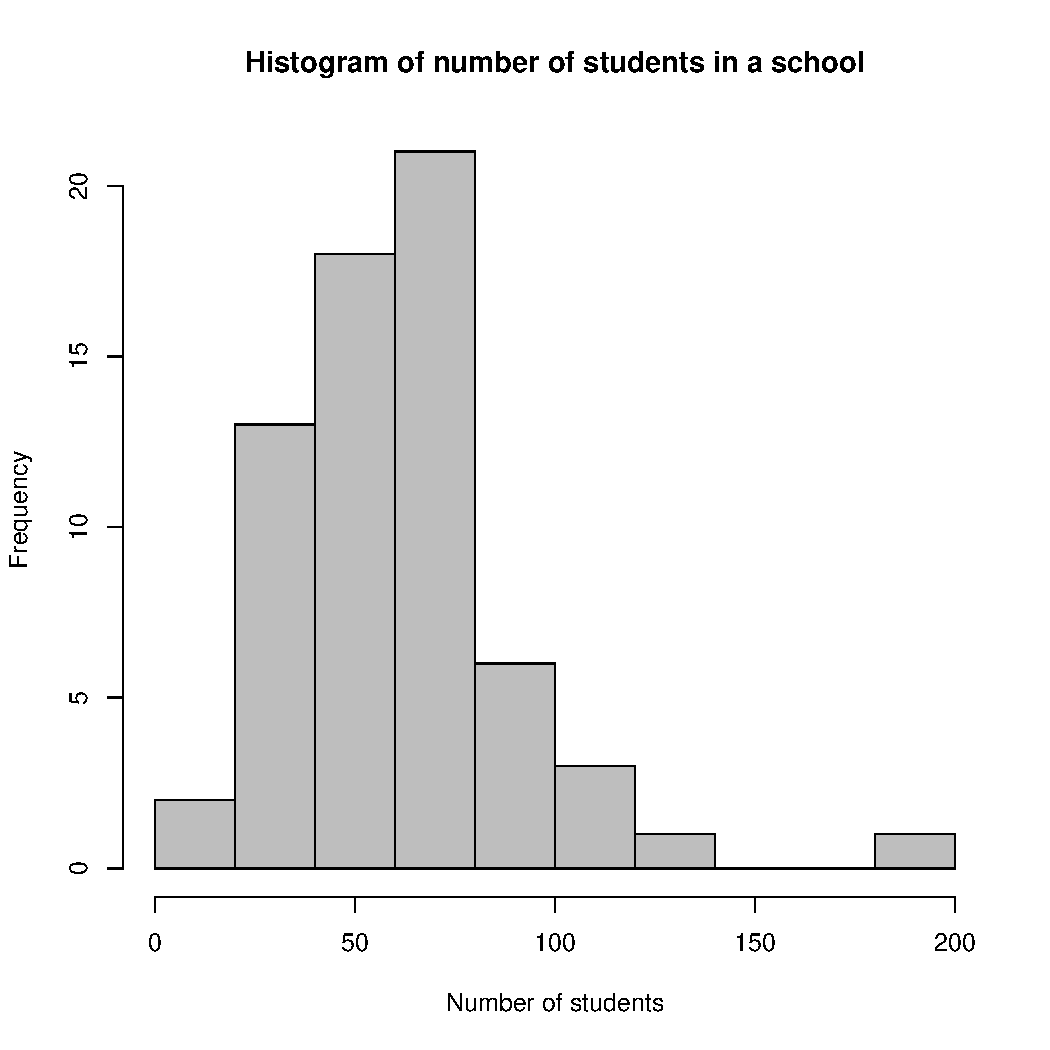
\includegraphics[width = 4in]{figures/histogram_1.pdf}
\caption{}
\label{hist1}
\end{figure}

A few interesting features of the histogram/data:
\begin{itemize}
\item Center of mass around 60 students
\item One school with about 200 (198) students
\item One school with 2 students and one school with 8 students
\end{itemize}

\subsection{GCSE exam scores}
Creating the normalized exam score histogram was more straightforward. After a preliminary histogram, no outliers appeared, so I again used Scott's rule for the bin widths with the standard \verb|hist()| function:

\begin{figure}[H]
\centering
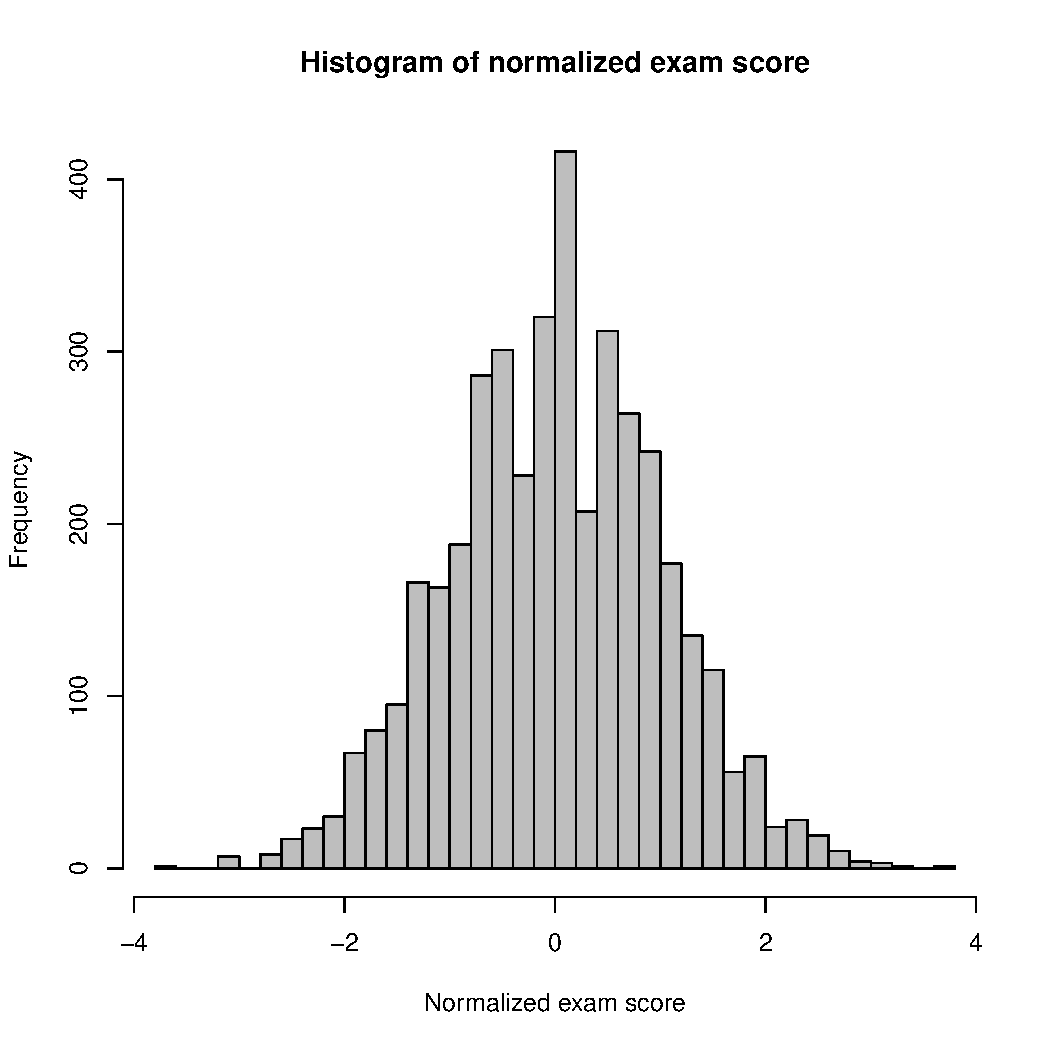
\includegraphics[width = 4in]{figures/histogram_2.pdf}
\caption{}
\label{hist2}
\end{figure}

As shown in Figure \ref{hist2}, the normalized exam scores appear mostly normally distributed. The maximum deviation from the mean exam score appears to be about 4 standard deviations in either direction. Another interesting aspect of the histogram are the two dips about 0.5 standard deviations from the mean exam score. These dips could be masked with wider bin widths (using Sturge's rule for the bins accomplishes this).

\subsection{Average LRT intake score for schools}
In this case again I had to manipulate the given data to cull out the observations for the histogram. To get the average London Reading Test intake scores for the schools, I first confirmed that the number of unique average scores was equal to the number of schools. With this assumption confirmed, I grabbed the unique school averages. To create the histogram, I again used Scott's rule
\begin{figure}[H]
\centering
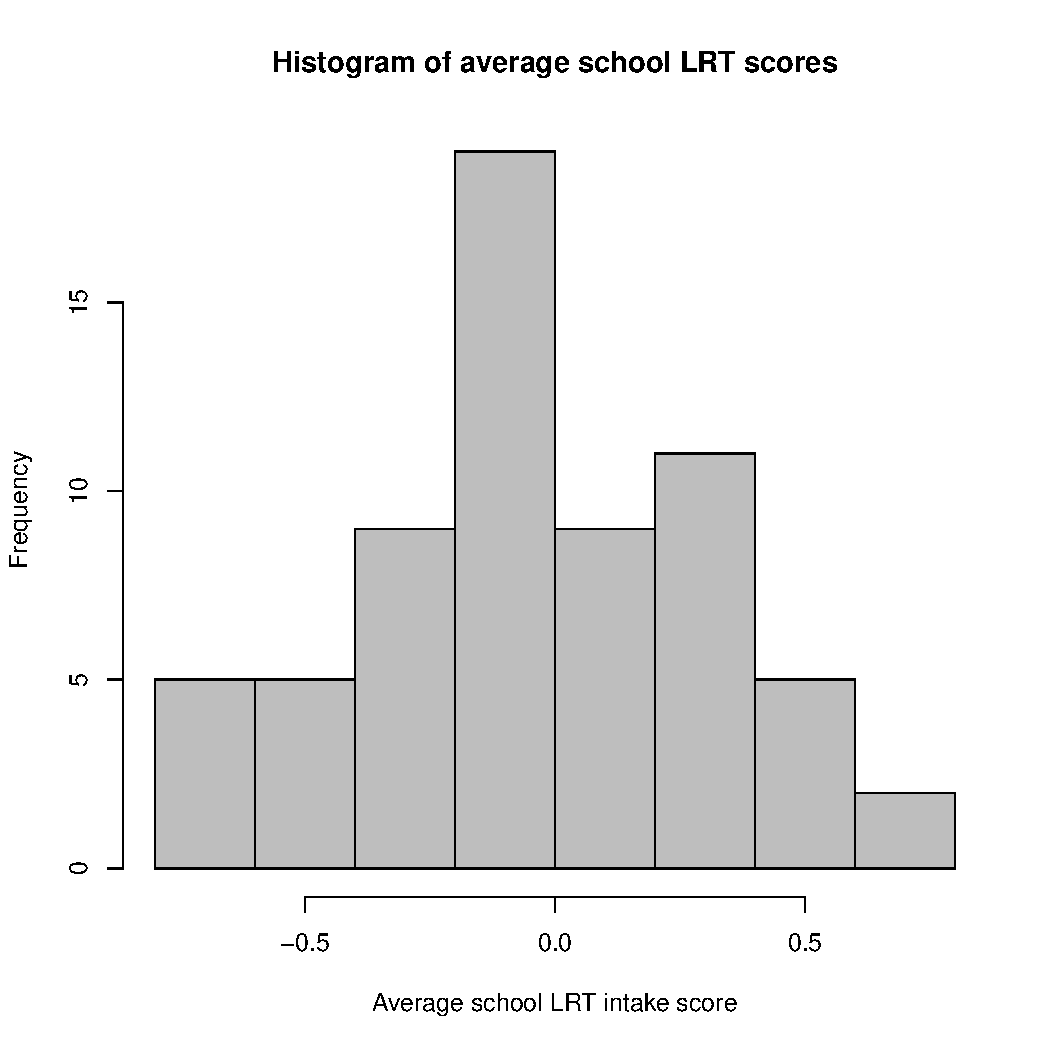
\includegraphics[width = 4in]{figures/histogram_3.pdf}
\caption{}
\label{hist3}
\end{figure}

Figure \ref{hist3} shows that, first, the observations reported are likely normalized test scores (unless students can get negative scores and the average score is magically 0). Next, while the scores are standardized, the distribution is a bit flat overall. The distribution is also fairly compressed. Compared to the standardized GCSE exam scores, the intake scores were at most 0.75 standard deviations away from the mean score. This might be a product of the exam itself. Finally, there appears to be a fairly large bump around the mean LRT intake score.

\subsection{Standardized LRT intake scores}
Requiring not pre manipulation, I plotted the standardized LRT intake scores for each student. The result, shown in Figure \ref{hist4} shows that the standardized scores appear normally distributed, with a few dips and a sharp drop over 1 standard deviation below the mean score. While no scores were below three standard deviations from the mean, there appear to be a small bump of scores above three standard deviations from the mean.

\begin{figure}[H]
\centering
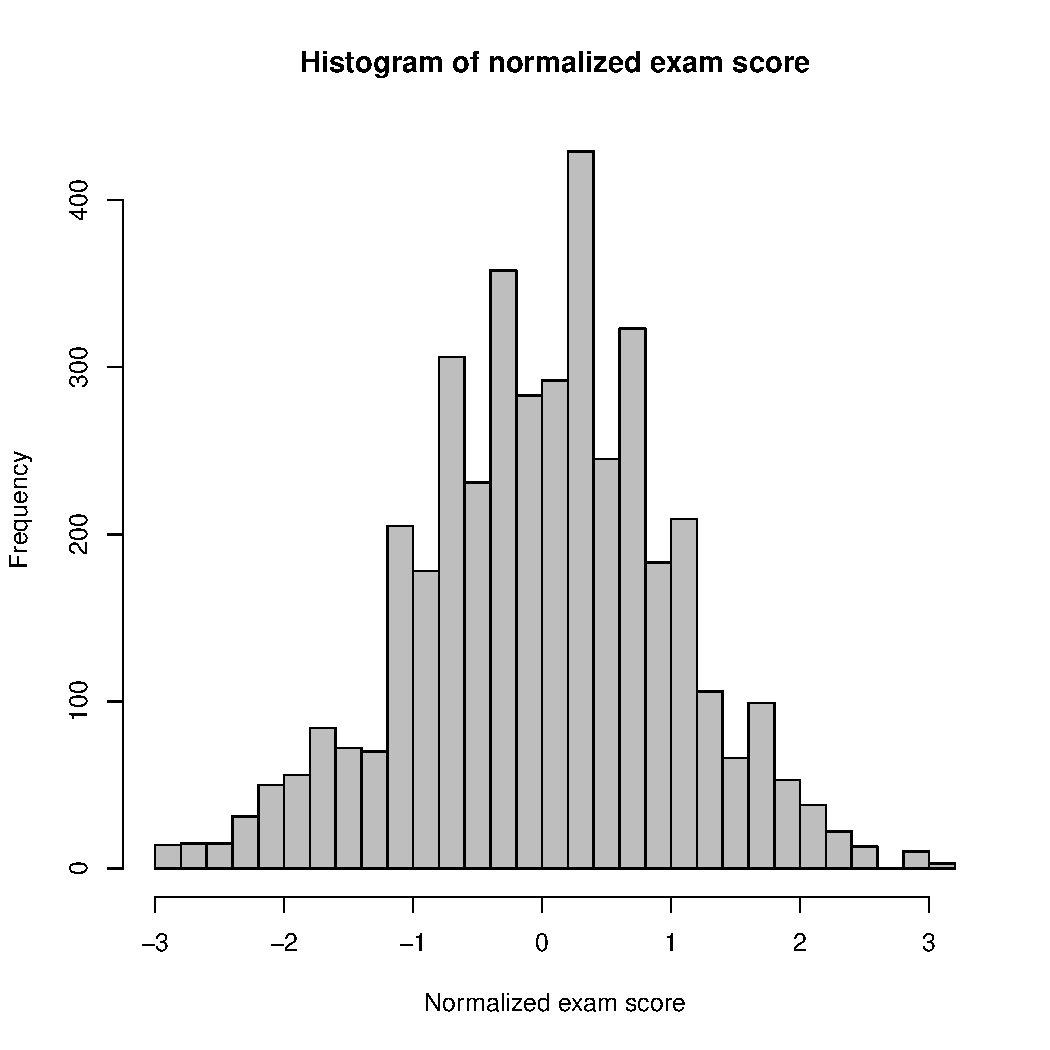
\includegraphics[width = 4in]{figures/histogram_4.pdf}
\caption{}
\label{hist4}
\end{figure}

\subsection{School gender types}
To make a table of the school gender type values, I used the standard R \verb|table()| function. The result in Table \ref{tab1} shows that over a fourth of the schools are girls-only, over half of the schools are mixed, and only about an eighth of the schools are boys-only. This imbalance could lead to issues using school gender type as a regressor.

\begin{table}[H]
\centering
\caption{School gender type}
\label{tab1}
\begin{tabular}{@{}  c c c@{}}
\textbf{Mixed} & \textbf{Boys} & \textbf{Girls} \\\midrule
 2169  & 513 & 1377 \\
\bottomrule
\hline
\end{tabular}
\end{table}

\subsection{Verbal reasoning subscores at intake}
As with school gender types, I used the R \verb|table()| function to generate the results in Table \ref{tab2}. Also similar to Table \ref{tab1}, the results are split with over half in one category (mid 50\%), over a fourth in another (top 25\%), and over an eighth in the last category (bottom 25\%). If overlap of the categories is also skewed, we could end up with very few data points for a combination such as ``students in an all boys school who performed in the bottom 25\% for VR intake".

\begin{table}[H]
\centering
\caption{Student verbal reasoning subscores at intake}
\label{tab2}
\begin{tabular}{@{}  c c c@{}}
\textbf{bottom 25\%} & \textbf{mid 50\%} & \textbf{top 25\%} \\\midrule
640     &  2263     &  1156 \\
\bottomrule
\hline
\end{tabular}
\end{table}

\subsection{Overall LRT scores at intake}
Unlike Table \ref{tab2}, the overall LRT scores show a flipped trend in Table \ref{tab3}, where over a fourth of the data are for students in the bottom 25\% and just over an eighth are in the top 25\%. As these screwed distributions continue to stack up, concern about a lack of data for a cross-section of the data points grows.

\begin{table}[H]
\centering
\caption{Student overall London Reading Test scores at intake}
\label{tab3}
\begin{tabular}{@{}  c c c@{}}
\textbf{bottom 25\%} & \textbf{mid 50\%} & \textbf{top 25\%} \\\midrule
      1176   &    2344     &   539 \\
\bottomrule
\hline
\end{tabular}
\end{table}


\subsection{Student's gender}
Table \ref{tab4} shows there are about 50\% more female students in the study than male students. While the other factor regressors have had three levels, this factor has two levels. This asserts that the variance in the regression parameter will be more impacted by skew in the category counts.

\begin{table}[H]
\centering
\caption{Student gender}
\label{tab4}
\begin{tabular}{@{}  c c @{}}
\textbf{Female} & \textbf{Male} \\\midrule
2436 & 1623\\
\bottomrule
\hline
\end{tabular}
\end{table}

\subsection{Type of schools}
Table \ref{tab5} represents a partial aggregation of the school gender type data. The mixed value is the same between the two factors and the ``single" value is the sum of the schools which are boys-only or girls-only. This factor is more balanced than the rest.

\begin{table}[H]
\centering
\caption{Student gender}
\label{tab5}
\begin{tabular}{@{}  c c @{}}
\textbf{Mixed} & \textbf{Single} \\\midrule
2169 &1890 \\
\bottomrule
\hline
\end{tabular}
\end{table}

\section{Intercept-only regression (GCSE exam scores): ``...Intercepts.R"}
\subsection{Complete pooling}
To find the complete pooling intercept, I conducted a regular linear regression with only a constant independent variable with students GCSE exam scores as the dependent variable (ignoring the clustering of students by schools). The result, as expected, is simply the mean of all the student normalized exam scores which is (about) $0$ which is also expected since the exam scores are normalized. To display the result, I plotted the complete pooling mean across each schools data with quartile ranges as shown in Figure \ref{complete pool}. As in the lecture notes, the red dashed line is the complete-pooling mean and the solid blue lines represent a 95\% confidence interval on the complete-pooling intercept in  predicting the school-level intercepts (means). As shown the confidence interval is extremely small relative to the deviations in school-level exam scores.

\begin{figure}[H]
\centering
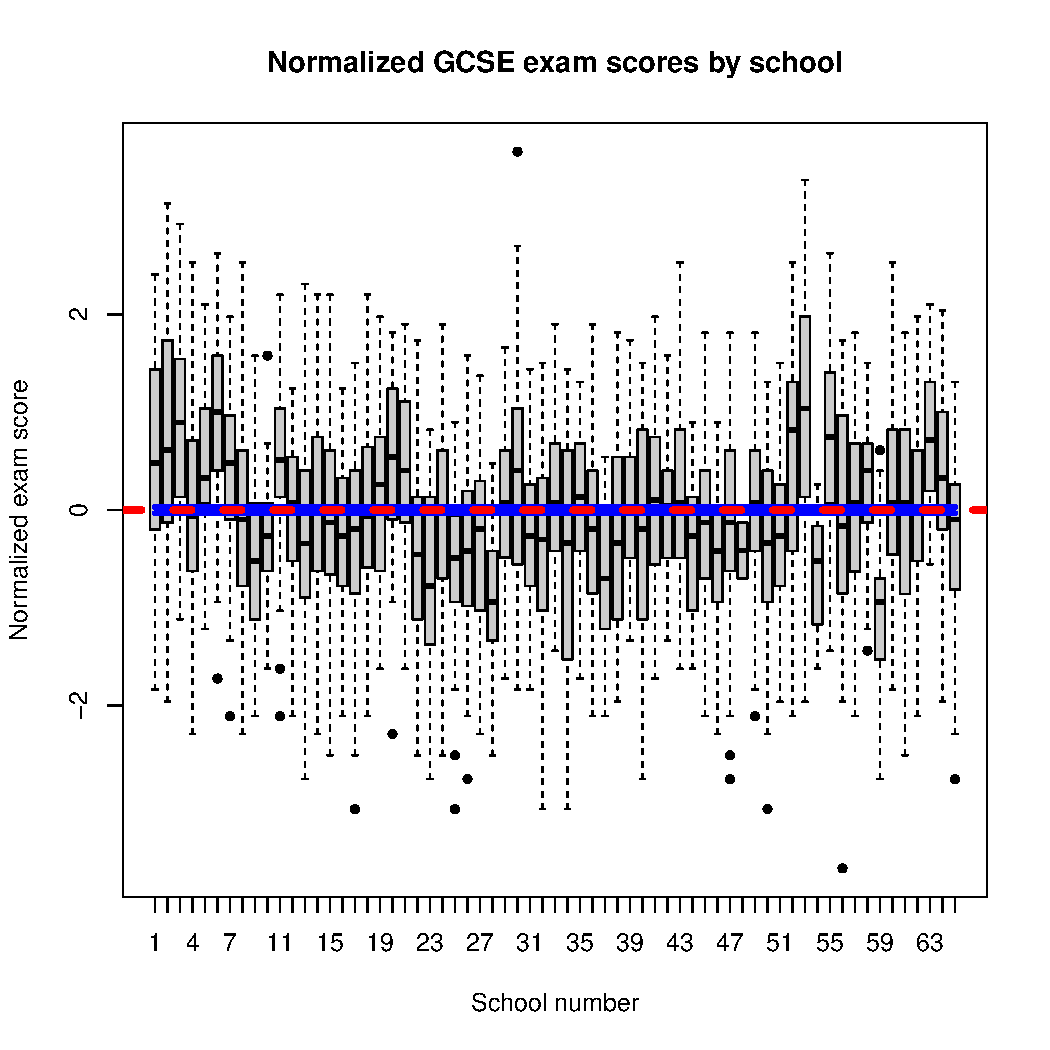
\includegraphics[width = 6in]{figures/complete_pooling.pdf}
\caption{Complete pooling intercept-only regression}
\label{complete pool}
\end{figure}

\subsection{No pooling}
To perform the no pooling intercept-only regression on GCSE exam scores, I tried both of the methods used in the notes. The first involved an individual regression on the data from each school using R's \verb|lapply()| function. While this was efficient, it would be difficult to grab the coefficients from the list result. For the sake of easier access to the regression coefficients, I then did a single regression (with a 0 intercept) where the only regressor was a dummy variable for the school number. The coefficients of that single regression are the school-level normalized exam score means. To display the results, I constructed a histogram of the school-level scores and a plot of the standard errors of the means as a function of their value which are both shown in Figure \ref{no pooling}. While most of the normalized scores are within 0.5 standard deviations from the mean, about 15 schools are more than 0.5 standard deviations from the mean exam score. There are also two large frequency bumps: one around -0.25 SD from the mean score and another around the mean exam score (though because of the bin placement it appears as though those values are greater than the mean). The standard errors hover between 0.05 and 0.15 standard deviations with a couple of schools which have SEs larger than 0.25.

\begin{figure}[H]
\centering
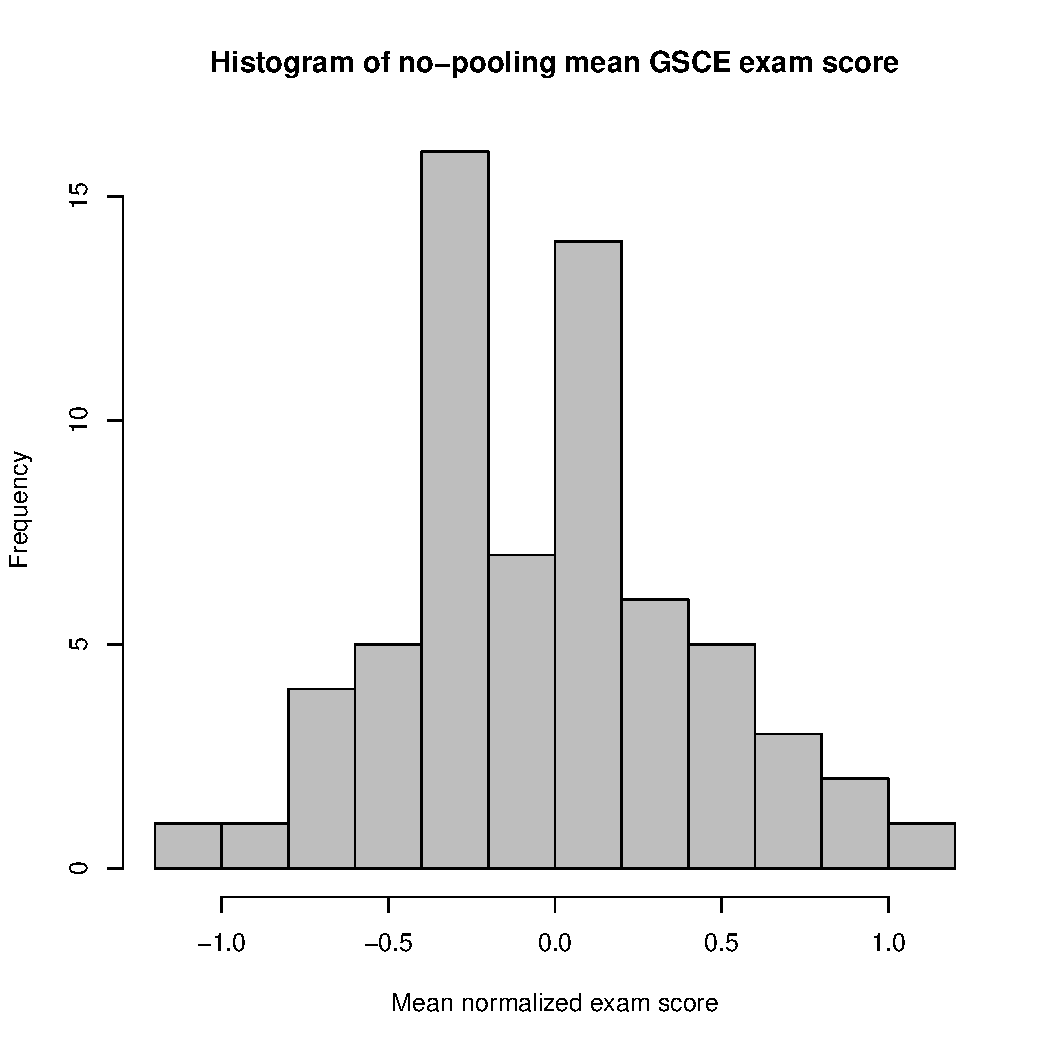
\includegraphics[width = 4in]{figures/no_pooling.pdf}
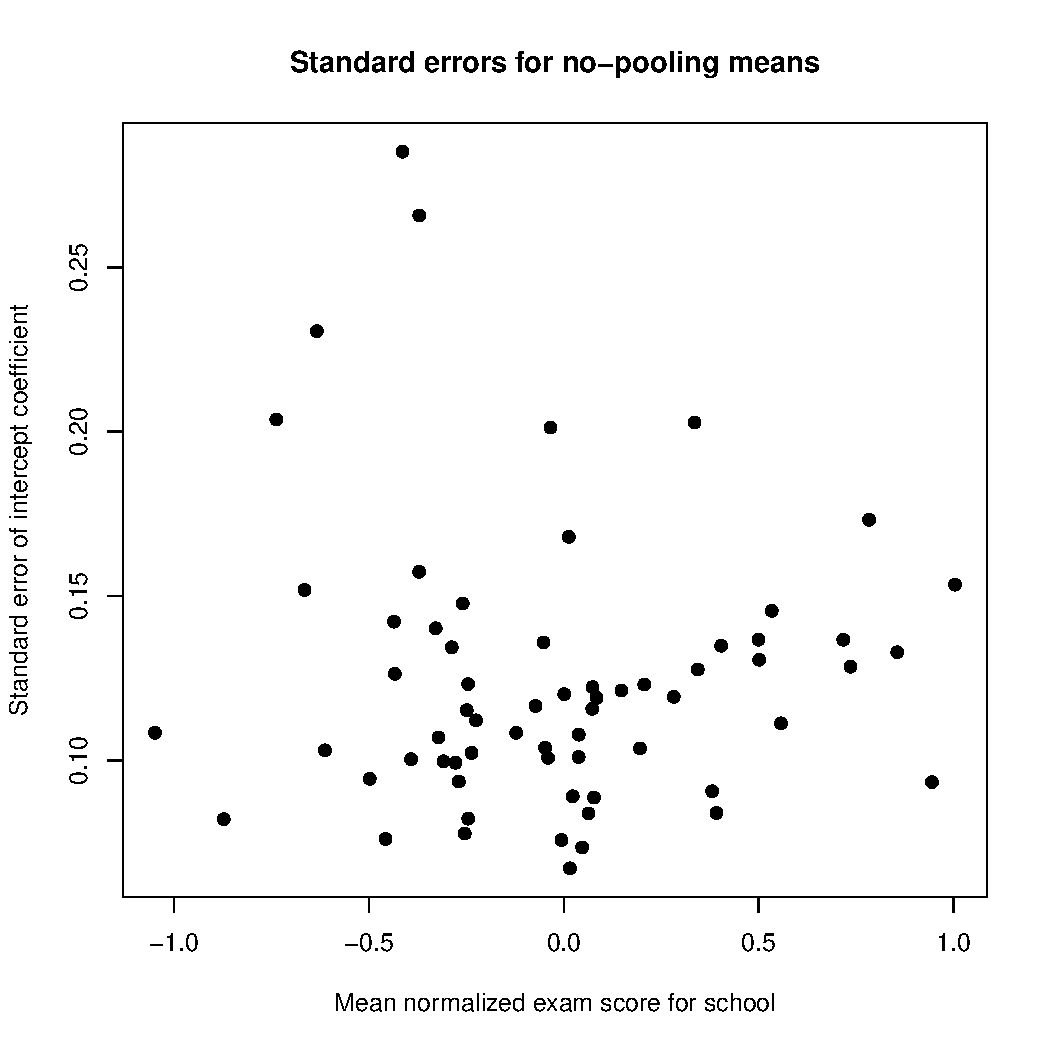
\includegraphics[width = 4in]{figures/no_pooling_se.pdf}
\caption{Frequency and standard errors for mean exam scores by school}
\label{no pooling}
\end{figure}

\subsection{Partial pooling}
To conduct partial pooling regressions using only an intercept, I used the \verb|lmer()| function of the "arm" package which allows for mixed effects. I then produced a histogram for the partial pooling normalized mean exam scores by school, shown in Figure \ref{partial pooling}. The result looks similar to the distribution of the no pooling school means, with deviations above and below the no pooling distribution as the scores are farther from the mean. To better understand the differences in the distributions, I created the QQ plot in Figure \ref{QQ} which confirms that:
\begin{itemize}
\item For schools with mean normalized exam scores lower than the complete pooling mean (0), the partial pooling mean was higher (pulling the values closer to the complete pooling mean)
\item For schools with mean normalized exam scores higher than the complete pooling mean, the partial pooling mean was lower (again, pulling the values closer to the complete pooling mean)
\end{itemize}

This difference is expected because even if the sample size in a given school is large\footnote{Data set is finite so large $< \infty$}, it will still be marginally shifted towards the complete pooling estimate.


\begin{figure}[H]
\centering
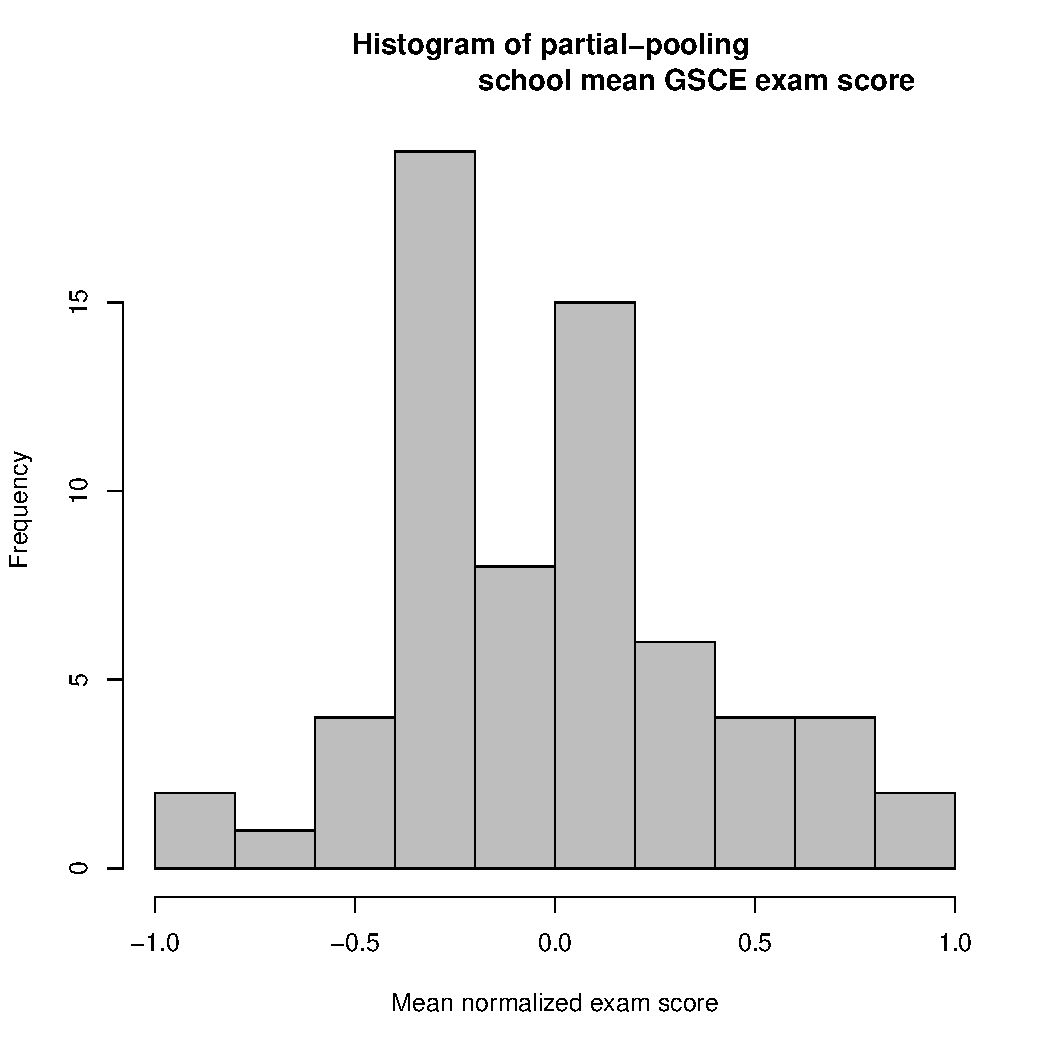
\includegraphics[width = 4in]{figures/partial_pooling.pdf}
\caption{}
\label{partial pooling}
\end{figure}

\begin{figure}[H]
\centering
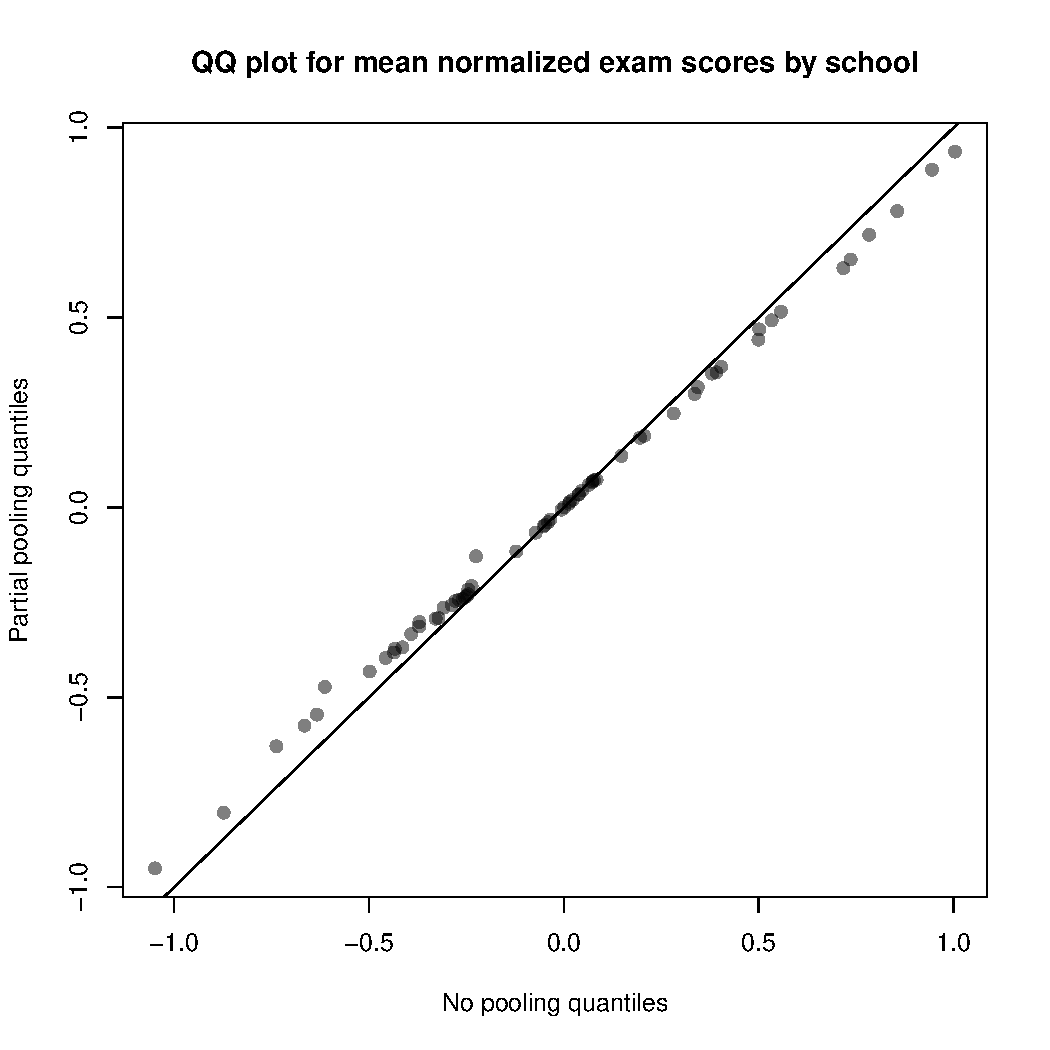
\includegraphics[width = 4in]{figures/no_vs_partial.pdf}
\caption{}
\label{QQ}
\end{figure}

\begin{figure}[H]
\centering
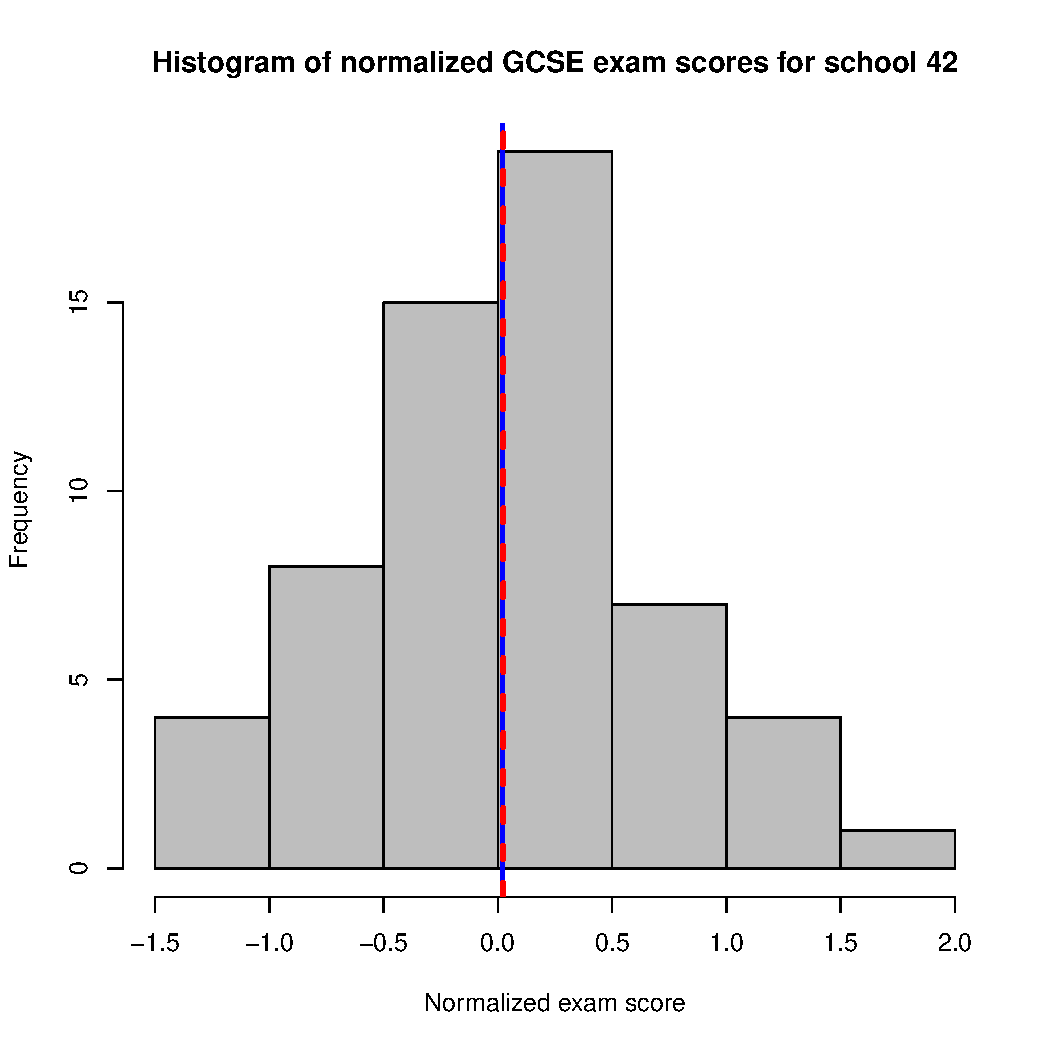
\includegraphics[width = 4in]{figures/42.pdf}
\caption{Partial pooling (blue) and no pooling (red) intercepts for school \# 42}
\label{42}
\end{figure}

\subsection{Example school}
To visualize the difference between the no pooling and partial pooling mean, I pulled the data for school number 42 and created a histogram of the normalized GCSE test scores with vertical lines marking the no pooling and partial pooling intercepts (means). In this case, the fitted intercepts were almost the same, as shown in Figure \ref{42} with the partial pooling slightly closer to 0 than the no pooling (as expected).

\section{}
As indicated in the lecture notes, the high-level purpose of partial pooling, in this case, is to account for three things:
\begin{itemize}
\item The variance of exam scores within each school
\item The variance of exam scores between schools
\item The number of students in each school
\end{itemize}

Given these figures, a partially pooled school intercept will be closer to complete pooling when the number of students in the school is less than the ratio of the variance of exam scores within the school to the variance of the exam scores between schools. When the number of students in the school is greater than this ratio, the partially polled school intercept will be closer to the no pooling value. This relationship is intuitive because, all else the same:
\begin{itemize}
\item A school with a greater number of students gives us more confidence that the mean value for the school is representative (no pooling)
\item A school with less variance in the exam scores gives us confidence in the same direction (no pooling)
\item When the variation between schools is smaller, we tend to think that there is little connection between the mean score and the school, so we favor the pooled result
\end{itemize}

\section{Adding standardized intake LRT score: ``...LRT.R"}
\subsection{Complete pooling}
To add the student’s standardized intake score on the London Reading Test at age 11 as a predictor to the complete pooling regression, I simply added the variable to my regular linear regression \verb|lm()| model. This resulted in an intercept about 10 times the original intercept without the LRT score (-0.0012 vs -0.00011) but clearly the final value is still very close to $0$.

\subsection{No pooling}
Using the same dummy variable approach, I added \verb|standLRT| to the linear regression model. I then re-created the histogram of intercept values for comparison with the previous no pooling regression. The result in Figure \ref{LRT no pooling} shows a significantly different intercept value distribution. In comparison to the regression without the LRT score, the distribution of intercept values is shifted right substantially.

\begin{figure}[H]
\centering
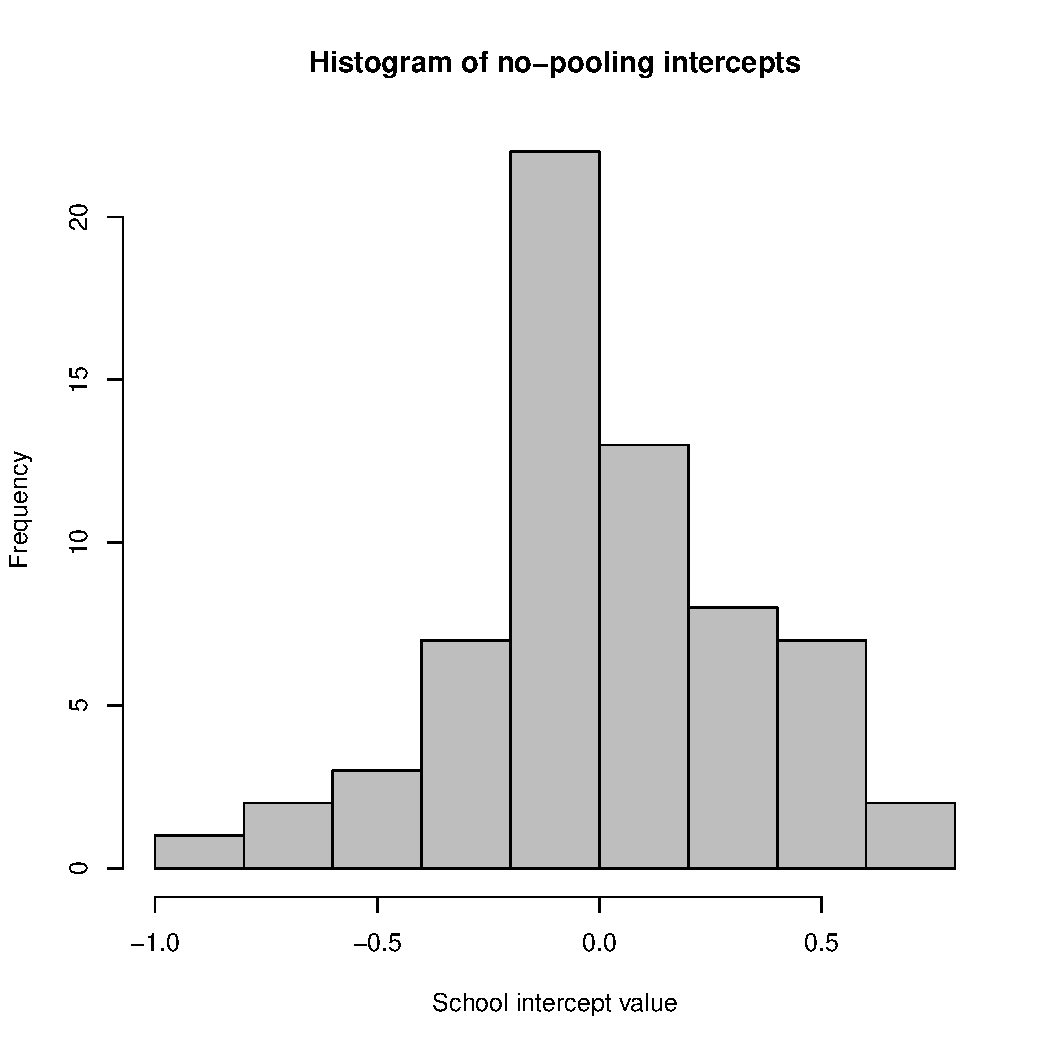
\includegraphics[width = 4in]{figures/no_pooling_LRT.pdf}
\caption{}
\label{LRT no pooling}
\end{figure}

\begin{figure}[H]
\centering
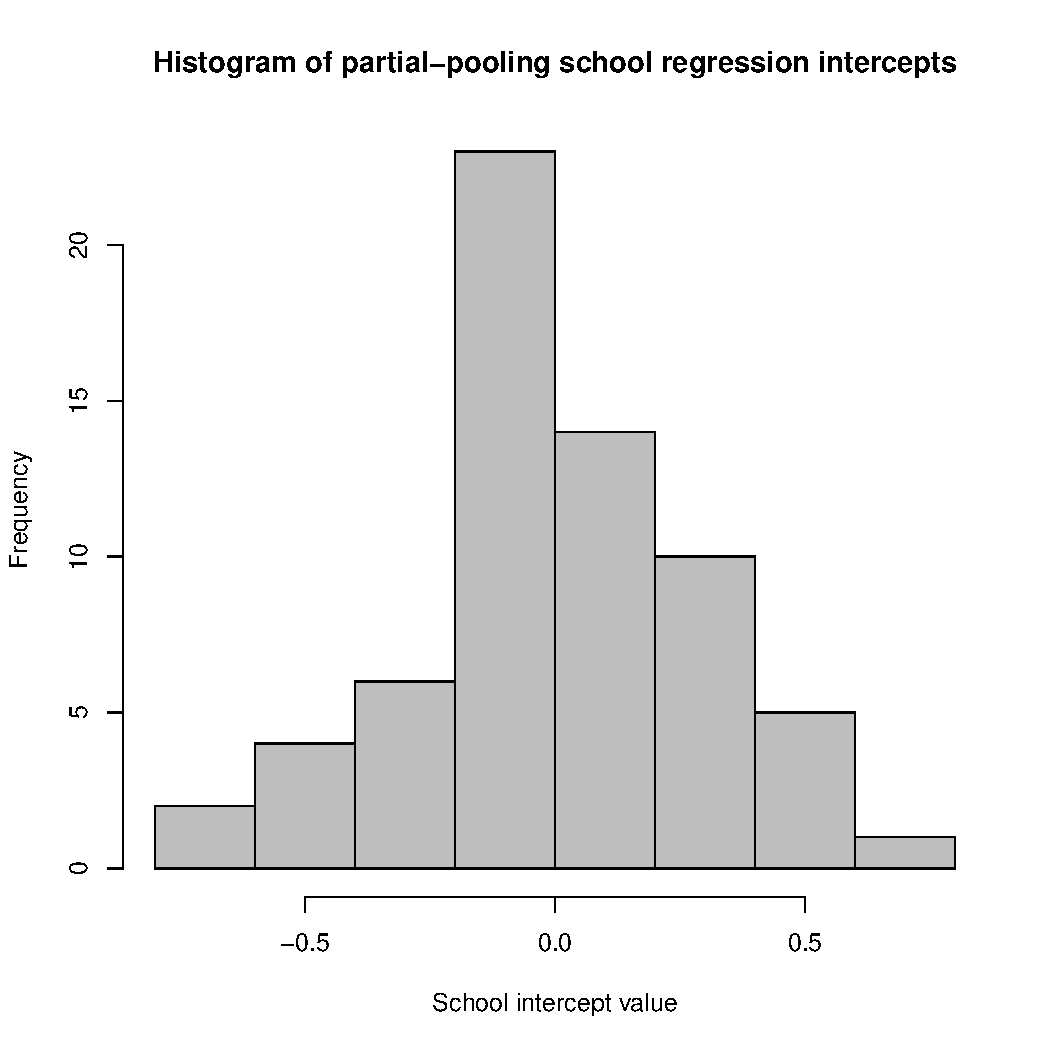
\includegraphics[width = 4in]{figures/partial_pooling_LRT.pdf}
\caption{}
\label{LRT partial}
\end{figure}

\subsection{Partial pooling}
For partial pooling, I again utilized the \verb|lmer()| function and added the \verb|standLRT| variable to the regression. To display the changes to the intercepts as this predictor is added, I again constructed a histogram of the intercept values which is shown in Figure \ref{LRT partial}. The results show a similar change to that of the new no pooling regression (rightward shift). 

\subsection{Regression comparison}
To compare these new regressions, I looked at both the distribution of intercept values and the estimated coefficients for the LRT scores. To compare the distribution of intercept values, I again used a QQ plot, but this time with the complete pooling intercept value added as a single dashed black line. The QQ plot is shown in Figure \ref{compare LRT} and indicates that, while the distributions have become more similar for a larger span around the median, the deviations have increased around the tails in the same general trends as before.

\begin{figure}[H]
\centering
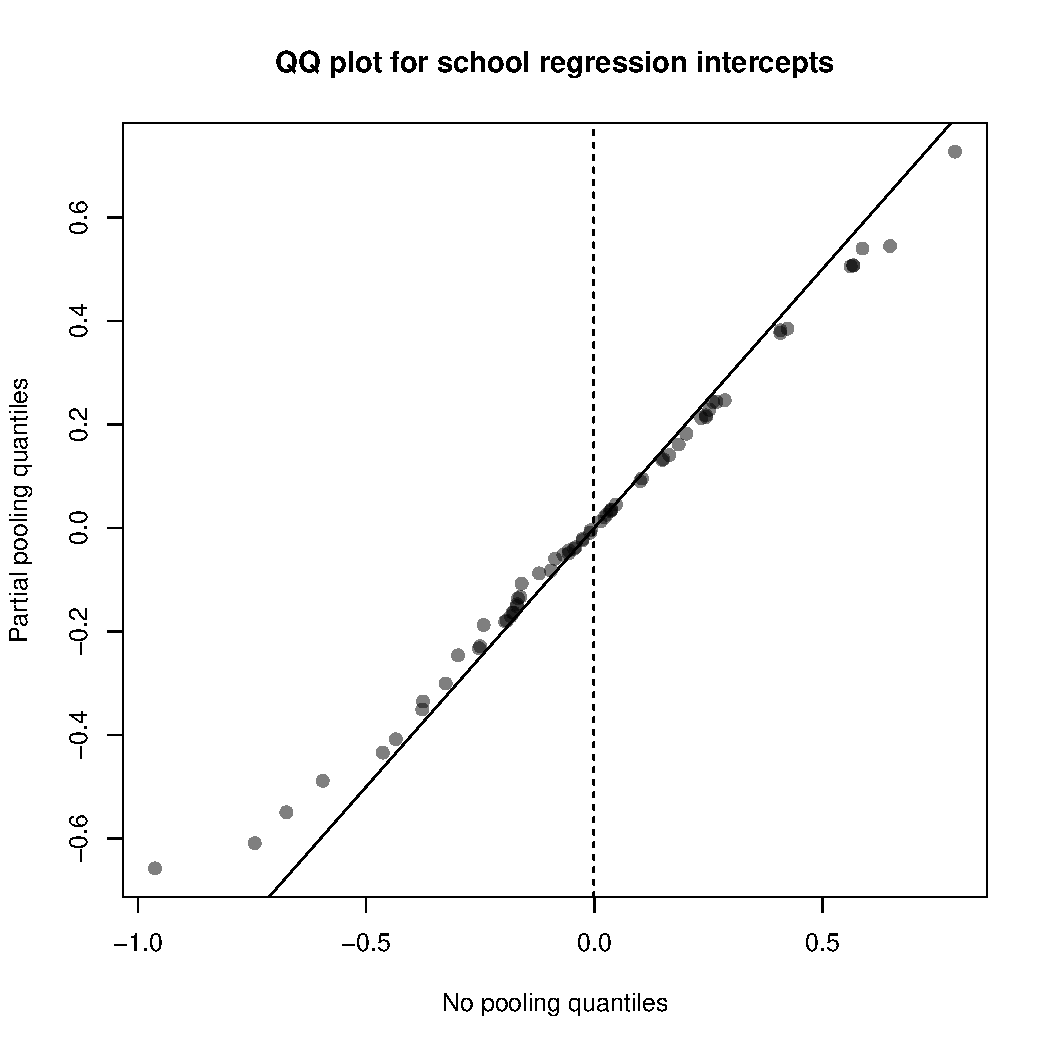
\includegraphics[width = 4in]{figures/comparison_LRT.pdf}
\caption{}
\label{compare LRT}
\end{figure}

The LRT score coefficients for each regression are shown in Table \ref{standLRT}. While the values are similar, the complete pooling coefficient is about $0.03$ larger than the no pooling coefficient. As the lecture notes mention, this indicates that there is some correlation between the LRT intake scores and the school-level GCSE scores (intercepts). We should be concerned about this correlation because if it is not accounted for, we may conclude that GCSE scores are more dependent on the school than they actually are.

\begin{table}[H]
\centering
\caption{}
\label{standLRT}
\begin{tabular}{@{}  l c @{}}
\textbf{Regression} & \textbf{standLRT coefficient} \\\midrule
Complete pooling &  0.595\\
Partial pooling & 0.563\\ 
No pooling & 0.559\\ 
\bottomrule
\hline
\end{tabular}
\end{table}

\section{Group-level predictor: ``...LRT2.R"}
To add the average London Reading Test intake score for the school as a group-level predictor in a multi-level model, I again used the \verb|lmer| function and added the \verb|schavg| variable as a regressor. This produced the distribution of intercept values shown in Figure \ref{groupie}.

\begin{figure}[H]
\centering
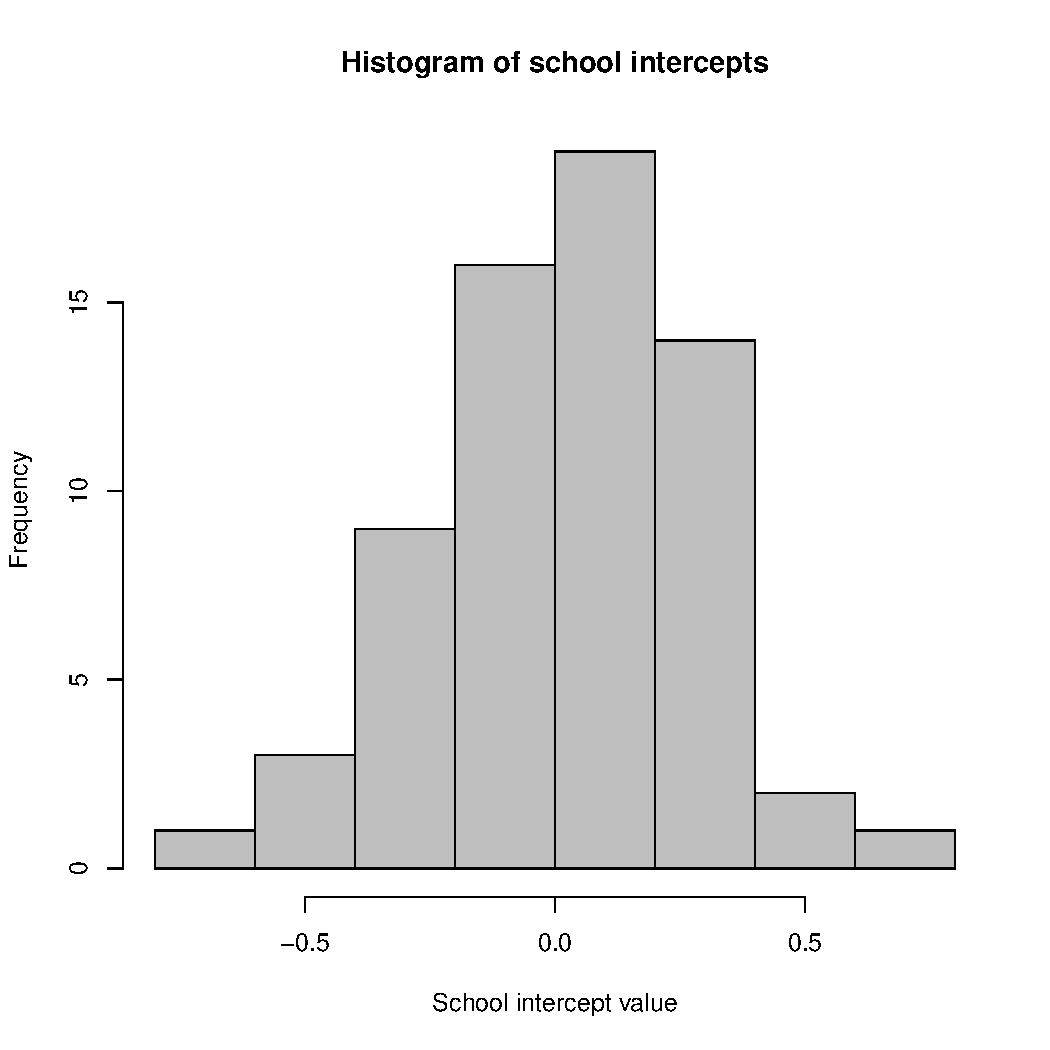
\includegraphics[width = 4in]{figures/group_level.pdf}
\caption{}
\label{groupie}
\end{figure}

As shown above, the spread of the distribution in the multi-level model is smaller than in any of the previous pooling regressions. Overall, adding in the school average LRT scores reduced the variance of the school intercept values from 0.094 (partially pooled) to 0.079. At this point I realized that if I were to try and complete the rest of the questions on-time, I would be going through the paces without learning anything.\footnote{I also re-read the syllabus!}

\setcounter{section}{10}
\section{}
Econometricians, statisticians, and machine learning researchers are hungry because when they cook together, the econometrician has to log every step, the ML researcher requires supervision, and the statistician can't make sense of what either of them are saying.


\section{}
possible issues:
- selection bias (students who did not have results for both intake measures were different than students who did)
- students who did not take an exam got a score of 0. I wonder how this impacts the regression? 0 is lower than a score of 1, but these results can't be ordered as such?

\end{document}
